\section{Analyse et reflexions }
\subsection{User Stories}

\subsubsubsection{Exemple}
\begin{figure}[H]
    \centering
    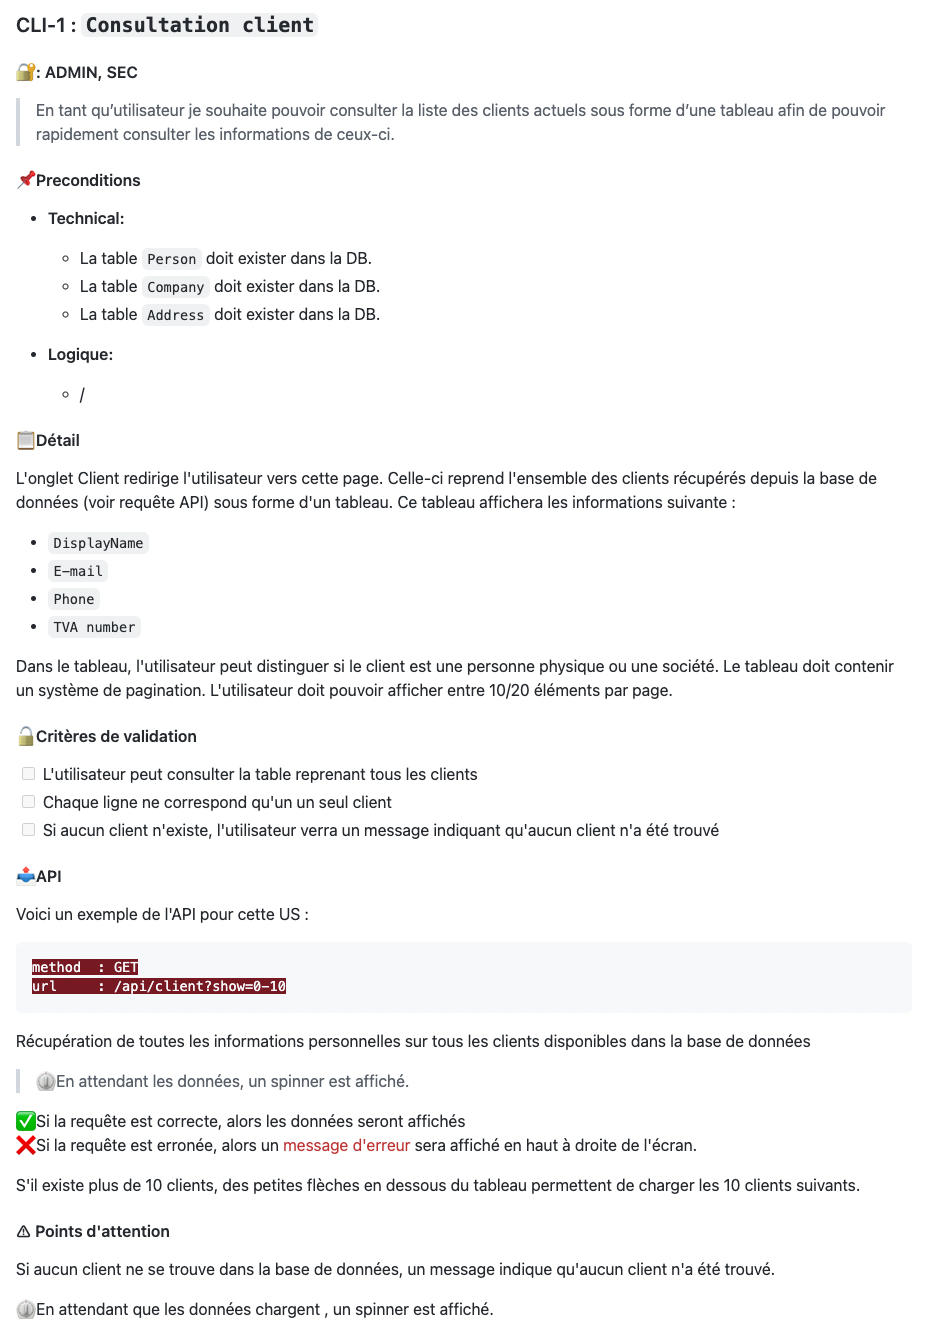
\includegraphics[scale=0.85]{img/userstories.png}
    \caption{Exemple de description de User Story}
    \label{Description user story}
  \end{figure}
\subsection{Liste des fonctionnalités dévélopées}
Toutes les fonctionnalités prévues pour le projet ont été réalisées. 
Ci-dessous, vous pouvez voir une vue non-détaillée des fonctionnalités implémentées.

\textbf{Utilisateur}
\begin{todolist}
    \item[\done] U01 - Connexion utilisateur
    \item[\done] U02 - Consulter les utilisateurs
    \item[\done] U03 - Ajouter un nouveau utilisateur
    \item[\done] U04 - Modifier utilisateur
    \item[\done] U05 - Supprimer utilisateur 
\end{todolist}

\textbf{Clients}
\begin{todolist}
    \item[\done] CLI-1 : Consultation la listes des clients
    \item[\done] CLI-2 : Consulter le détail d’un client
    \item[\done] CLI-3 : Ajouter un nouveau client
    \item[\done] CLI-4 : Modification d'un client
    \item[\done] CLI-5 : Supprimer un client
    \item[\done] CLI-6 : Rechercher un client
    \item[\done] CLI-7 : Trier la liste des clients 
\end{todolist}

\textbf{Projets}
\begin{todolist}
    \item[\done] PRJ-1 : Consulter la listes des projets
    \item[\done] PRJ-2 : Consulter le détail d’un projet
    \item[\done] PRJ-3 : Rechercher un projet
    \item[\done] PRJ-4 : Filtrer un projet
    \item[\done] PRJ-5 : Ajouter d’un projet
    \item[\done] PRJ-6 : Modifier le contenu d’un projet
    \item[\done] PRJ-7 : Supprimer un projet

\end{todolist}

\textbf{Matériel}
\begin{todolist}
    \item[\done] MA-1 : Consulter la liste de matériel disponible
    \item[\done] MA-2 : Consulter le détail d’un matériel
    \item[\done] MA-3 : Ajouter d'un matériel à un projet
    \item[\done] MA-4 : Rechercher d'un matériel 
    \item[\done] MA-5 : Désaffecter un matériau d'un projet
    \item[\done] MA-6 : Modifier un matériel
    \item[\done] MA-7 : Supprimer du matériel

\end{todolist}

\textbf{Devis}
\begin{todolist}
    \item[\done] DE-1 : Consultation devis
    \item[\done] DE-2 : Générer un devis
    \item[\done] DE-3 : Consulter le détail d'un devis 
    \item[\done] DE-4 : Consulter les devis appartenant à un projet
    \item[\done] DE-5 : Envoyer devis par mail
    \item[\done] DE-6 : Recherche un devis
    \item[\done] DE-7 : Trier la liste des devis
\end{todolist}

\textbf{Factures}
\begin{todolist}
    \item[\done] FA-1 : Consultation facture
    \item[\done] FA-2 : Générer une facture
    \item[\done] FA-3 : Consulter détail d'une facture
    \item[\done] FA-4 : Consulter les factures appartenant à un projet
    \item[\done] FA-5 : Envoyer une facture par mail
    \item[\done] FA-6 : Télécharger facture
    \item[\done] FA-7 : Recherche une facture
    \item[\done] FA-8 : Trier la liste des factures

\end{todolist}